% Provenance (never printed): NSI premiere "Architectures materielles" (circuits combinatoires, ALU), PCSI option
% informatique / L1 architecture (additionneurs, multiplexeurs, bascules). See sources/book2/BRIEFS.md.
\chapter{From Gates to an Arithmetic Unit}\label{ch:g11:gates-to-arithmetic-unit}

Book 1 ended its tour of logic gates with a half adder: two bits in, their sum and their carry out. A processor adds
two numbers of $64$ bits each, billions of times a second, and it has no other material than such gates. This chapter
builds the missing steps one at a time: an adder for three bits, an adder for whole numbers, a circuit that chooses,
an \omterm{def:g11:gates-to-arithmetic-unit:alu}{arithmetic and logic unit} with its \omterm{def:g11:gates-to-arithmetic-unit:flag}{flags}, and finally a circuit that remembers. Each one is simulated in Python,
gate by gate, and checked on every input.

\begin{recall}
A gate computes one bit from one or two bits: NOT, AND, OR, XOR, and NOR, which is NOT OR. A half adder computes
$a + b$ for two bits: the sum bit is $a \oplus b$ and the carry is $a \wedge b$. De Morgan's laws turn an AND into an
OR of negations and back. A transistor works as a switch, which is how gates are built (Book 1, grade 9). On $n$ bits,
\omterm{def:g10:machine-integers:twos-complement}{two's complement} writes $-x$ as $2^n - x$ (the chapter on numbers in binary).
\end{recall}

The gates of the chapter are Python functions on the bits $0$ and $1$, in the module \code{gates.py}: \code{NOT(a)}
returns $1 - a$, \code{AND}, \code{OR} and \code{XOR} use Python's bitwise operators, and \code{NOR(a, b)} is
\code{NOT(OR(a, b))}. Every circuit below is written with these five functions only.

\begin{omfigure}
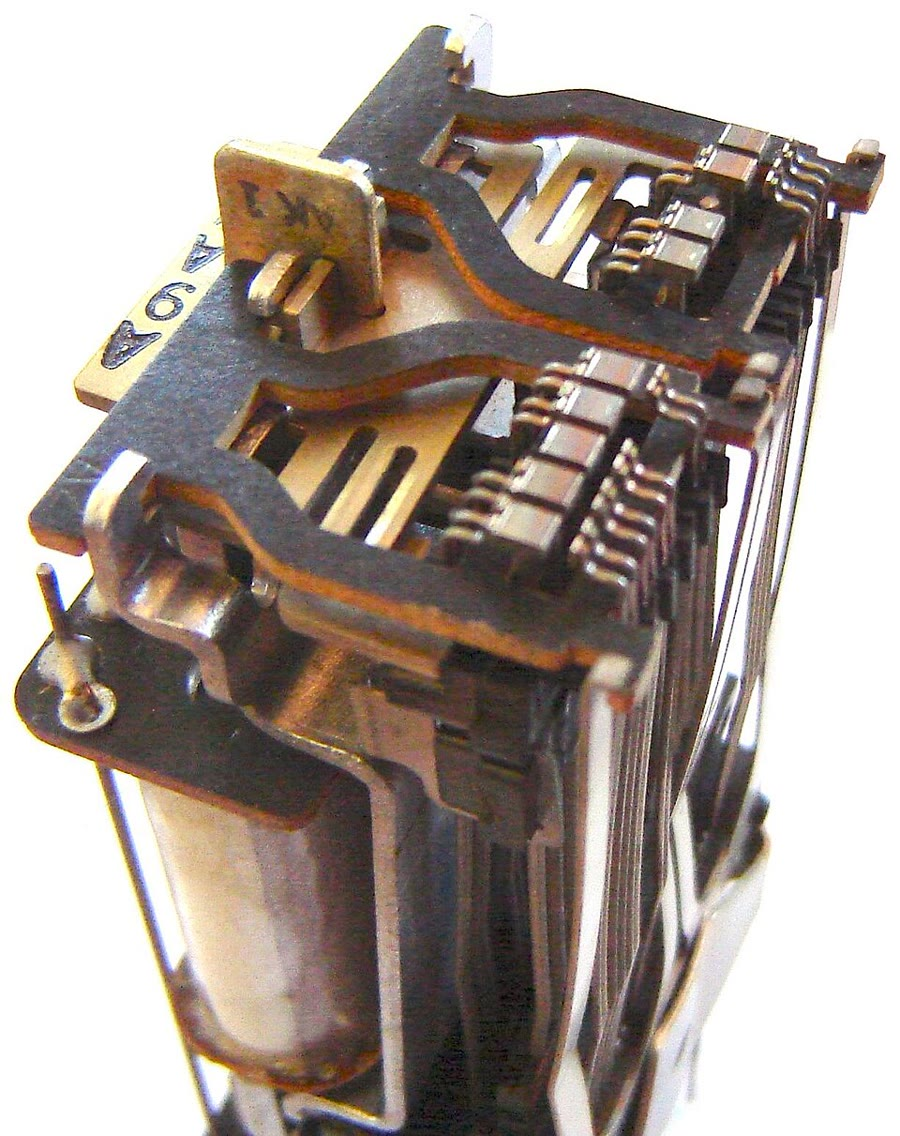
\includegraphics[width=0.3\linewidth]{images/book2/g11-relay.jpg}

{\small A relay: an electromagnet that pulls metal contacts open or shut, a switch worked by a current. Machines such
as the Harvard Mark II built their logic from relays before transistors replaced them (Book 1, grade 7).
Photograph: Duncan Smith, public domain.}
% ledger: g7:bug-1947
\end{omfigure}

\section{The full adder}\label{sec:g11:gates-to-arithmetic-unit:full-adder}

To add two numbers written in binary, each column adds three bits: the two digits of the column, and the carry from
the column on its right. The half adder takes only two.

\begin{definition}[Full adder]\label{def:g11:gates-to-arithmetic-unit:full-adder}
A \emph{full adder}\index{full adder} is a circuit with three input bits $a$, $b$, $c$ and two output bits $s$ and
$c'$ such that $a + b + c = 2c' + s$: $s$ is the sum bit, and $c'$ the carry out.
\end{definition}

A \omterm{def:g11:gates-to-arithmetic-unit:full-adder}{full adder} is made of two half adders and an OR gate. The first half adder adds $a$ and $b$, the second adds the
carry $c$ to their sum bit, and since the two carries cannot both be $1$, an OR combines them.

\begin{omfigure}
\begin{circuitikz}[font=\small, dot/.style={circle, fill, inner sep=0pt, minimum size=3pt}]
  \node[xor port] (x1) at (2.2,1.6) {};
  \node[and port] (a1) at (2.2,-0.8) {};
  \node[xor port] (x2) at (6.0,1.3) {};
  \node[and port] (a2) at (6.0,-0.1) {};
  \node[or port, anchor=in 1] (o) at ($(a2.out)+(1.2,0)$) {};
  \draw (-0.2,2.5) node[left] {$a$} -| (0.4,0) |- (x1.in 1);
  \draw (0.4,0) |- (a1.in 1);
  \draw (-0.2,2.1) node[left] {$b$} -| (0.8,0) |- (x1.in 2);
  \draw (0.8,0) |- (a1.in 2);
  \node[dot] at (0.4,0 |- x1.in 1) {}; \node[dot] at (0.8,0 |- x1.in 2) {};
  \draw (x1.out) -- node[above] {$p$} (4.0,0 |- x1.out) |- (x2.in 1);
  \draw (4.0,0 |- x1.out) |- (a2.in 1);
  \node[dot] at (4.0,0 |- x1.out) {};
  \draw (-0.2,-2.0) node[left] {$c$} -| (4.5,0) |- (x2.in 2);
  \draw (4.5,0) |- (a2.in 2);
  \node[dot] at (4.5,0 |- a2.in 2) {};
  \draw (a2.out) -- (o.in 1);
  \draw (a1.out) -- node[above, pos=0.15] {$g$} ([xshift=-5mm]o.in 2 |- a1.out) |- (o.in 2);
  \draw (x2.out) -- (x2.out -| o.out) -- ++(0.6,0) node[right] {$s$};
  \draw (o.out) -- ++(0.6,0) node[right] {carry out $c'$};
  \draw[omDef, dashed, rounded corners] (0.95,-1.55) rectangle (2.75,2.35);
  \node[omDef, font=\scriptsize, anchor=south] at (1.85,2.35) {half adder};
  \draw[omDef, dashed, rounded corners] (4.25,-0.85) rectangle (6.6,2.05);
  \node[omDef, font=\scriptsize, anchor=south] at (5.4,2.05) {half adder};
\end{circuitikz}

{\small A \omterm{def:g11:gates-to-arithmetic-unit:full-adder}{full adder}: two half adders and an OR gate, five gates in all. A dot marks where a wire branches; wires
that cross without a dot are not connected.}
\end{omfigure}

\omcode{code/grade-11/01-gates-to-arithmetic-unit/listings/full_adder.py}{1}{23}{The \omterm{def:g11:gates-to-arithmetic-unit:full-adder}{full adder}, checked on its
eight rows.}\label{lst:g11:gates-to-arithmetic-unit:full-adder}

\omoutput{code/grade-11/01-gates-to-arithmetic-unit/outputs/full_adder.txt}{The truth table: the two outputs, read
as a binary number $c's$, are $a + b + c$.}\label{out:g11:gates-to-arithmetic-unit:full-adder}

Eight rows are all the inputs there are, so the \code{assert} of line~22 proves the circuit correct: an
\emph{exhaustive} check. A circuit whose outputs depend only on its present inputs, as here, is called
combinational.

\begin{definition}[Combinational and sequential circuits]\label{def:g11:gates-to-arithmetic-unit:combinational}
A \emph{combinational circuit}\index{combinational circuit} computes its outputs from its present inputs only: the
same inputs always give the same outputs. A \emph{sequential circuit}\index{sequential circuit} also depends on what
happened before, because some of its outputs are fed back to its inputs: it has a memory.
\end{definition}

\section{Chaining adders}\label{sec:g11:gates-to-arithmetic-unit:ripple}

\begin{definition}[Ripple-carry adder]\label{def:g11:gates-to-arithmetic-unit:ripple}
A \emph{ripple-carry adder}\index{ripple-carry adder} on $n$ bits is a row of $n$ \omterm{def:g11:gates-to-arithmetic-unit:full-adder}{full adders}, one per column: the
adder of column $i$ adds $a_i$, $b_i$ and the carry $c_i$ from column $i - 1$, and passes its carry out $c_{i+1}$ to
column $i + 1$. The first carry $c_0$ is an input, usually $0$; the last, $c_n$, is the carry out of the sum.
\end{definition}

\begin{omfigure}
\begin{tikzpicture}[font=\small, fa/.style={draw, fill=omDef!8, minimum width=14mm, minimum height=11mm}]
  \foreach \i in {0,...,3} {
    \node[fa] (f\i) at (-2.6*\i,0) {FA};
    \draw[<-] ([xshift=-3mm]f\i.north) -- ++(0,0.6) node[above] {$a_{\i}$};
    \draw[<-] ([xshift=3mm]f\i.north) -- ++(0,0.6) node[above] {$b_{\i}$};
    \draw[->] (f\i.south) -- ++(0,-0.6) node[below] {$s_{\i}$};
  }
  \draw[<-, very thick, omThm] (f0.east) -- ++(0.8,0) node[right] {$c_0$};
  \foreach \i/\j in {0/1,1/2,2/3} \draw[->, very thick, omThm] (f\i.west) -- node[above] {$c_{\j}$} (f\j.east);
  \draw[->, very thick, omThm] (f3.west) -- ++(-0.8,0) node[left] {$c_4$};
\end{tikzpicture}

{\small A $4$-bit \omterm{def:g11:gates-to-arithmetic-unit:ripple}{ripple-carry adder}, drawn with the least significant column on the right, as numbers are written.
The carry chain, in red, crosses every \omterm{def:g11:gates-to-arithmetic-unit:full-adder}{full adder}: column $3$ cannot finish before column $0$ has.}
\end{omfigure}

The simulation keeps the bits of a number in a list, least significant first, so that index $i$ is the column of
weight $2^i$.

\omcode{code/grade-11/01-gates-to-arithmetic-unit/listings/ripple.py}{1}{30}{An $8$-bit adder from eight \omterm{def:g11:gates-to-arithmetic-unit:full-adder}{full
adders}.}\label{lst:g11:gates-to-arithmetic-unit:ripple}

\omoutput{code/grade-11/01-gates-to-arithmetic-unit/outputs/ripple.txt}{The carries are printed from $c_8$ down to
$c_0$, in the order of the bits.}\label{out:g11:gates-to-arithmetic-unit:ripple}

The second sum, $200 + 100 = 300$, does not fit in $8$ bits: the result is $300 - 256 = 44$ and the carry out is $1$,
which signals the overflow for numbers read without sign. The third sum fits without sign, $200$, but read in \omterm{def:g10:machine-integers:twos-complement}{two's
complement}, $100 + 100$ gives $-56$, a sign change no correct sum of two positive numbers can have. A signed overflow
happens exactly when the carry into the last column differs from the carry out of it, which is what line~28
computes.

The same adder subtracts. Flipping every bit of $b$ gives $2^n - 1 - b$; adding $1$ gives $2^n - b$, the \omterm{def:g10:machine-integers:twos-complement}{two's
complement} of $b$. So $a - b$ is $a + \overline{b} + 1$, modulo $2^n$, and the $+1$ costs nothing: it enters as the
first carry $c_0$.

\omcode{code/grade-11/01-gates-to-arithmetic-unit/listings/subtract.py}{1}{15}{Subtraction through the adder: flip,
and carry in $1$.}\label{lst:g11:gates-to-arithmetic-unit:subtract}

\omoutput{code/grade-11/01-gates-to-arithmetic-unit/outputs/subtract.txt}{The carry out of a subtraction is $1$
exactly when $a \ge b$: when it is $0$, the subtraction needed a borrow.}\label{out:g11:gates-to-arithmetic-unit:subtract}

\section{Choosing and decoding}\label{sec:g11:gates-to-arithmetic-unit:mux}

A processor computes several things at once and keeps one; it also has to turn a number, such as the number of a
register, into one wire among several. Two small circuits do these jobs.

\begin{definition}[Multiplexer, decoder]\label{def:g11:gates-to-arithmetic-unit:mux}
A \emph{multiplexer}\index{multiplexer} with $k$ select bits has $2^k$ data inputs and one output, equal to the
data input whose number is written by the select bits. A \emph{decoder}\index{decoder} with $k$ input bits has
$2^k$ outputs, of which exactly one is $1$: the one whose number is written by the inputs.
\end{definition}

The $2{:}1$ \omterm{def:g11:gates-to-arithmetic-unit:mux}{multiplexer} is $(\neg s \wedge x_0) \vee (s \wedge x_1)$: when $s = 0$ the first AND lets $x_0$ through
and the second gives $0$, and the reverse when $s = 1$. Three of them make a $4{:}1$ \omterm{def:g11:gates-to-arithmetic-unit:mux}{multiplexer}.

\begin{omfigure}
\begin{tikzpicture}[font=\small]
  \newcommand{\muxat}[2]{%
    \draw[fill=omMeth!12] (#2) coordinate (#1) -- ++(0,1.4) -- ++(0.9,-0.35) -- ++(0,-0.7) -- cycle;
    \node[font=\scriptsize] at ($(#1)+(0.2,1.05)$) {0};
    \node[font=\scriptsize] at ($(#1)+(0.2,0.35)$) {1};}
  \muxat{A}{0,1.5}
  \muxat{B}{0,-1.5}
  \muxat{C}{2.8,0}
  \foreach \m/\u/\v in {A/x_0/x_1, B/x_2/x_3} {
    \draw ($(\m)+(-0.9,1.05)$) node[left] {$\u$} -- ++(0.9,0);
    \draw ($(\m)+(-0.9,0.35)$) node[left] {$\v$} -- ++(0.9,0);
    \draw ($(\m)+(0.45,-0.6)$) node[below] {$s_0$} -- ++(0,0.78);
  }
  \draw ($(A)+(0.9,0.7)$) -| (2.3,1.05) -- (2.8,1.05);
  \draw ($(B)+(0.9,0.7)$) -| (2.3,0.35) -- (2.8,0.35);
  \draw (3.25,-1.5) node[below] {$s_1$} -- (3.25,0.18);
  \draw[->] (3.7,0.7) -- (4.6,0.7) node[right] {output};
\end{tikzpicture}

{\small A $4{:}1$ \omterm{def:g11:gates-to-arithmetic-unit:mux}{multiplexer} from three $2{:}1$ \omterm{def:g11:gates-to-arithmetic-unit:mux}{multiplexers}. The bit $s_0$ chooses within each pair, then $s_1$
chooses between the pairs: the output is $x_{2s_1 + s_0}$.}
\end{omfigure}

\omcode{code/grade-11/01-gates-to-arithmetic-unit/listings/mux.py}{1}{26}{\omterm{def:g11:gates-to-arithmetic-unit:mux}{Multiplexers} and a $2$-to-$4$
\omterm{def:g11:gates-to-arithmetic-unit:mux}{decoder}.}\label{lst:g11:gates-to-arithmetic-unit:mux}

\omoutput{code/grade-11/01-gates-to-arithmetic-unit/outputs/mux.txt}{The \omterm{def:g11:gates-to-arithmetic-unit:mux}{multiplexer} copies the chosen input; the
\omterm{def:g11:gates-to-arithmetic-unit:mux}{decoder} lights the chosen output.}\label{out:g11:gates-to-arithmetic-unit:mux}

\section{An arithmetic and logic unit}\label{sec:g11:gates-to-arithmetic-unit:alu}

\begin{definition}[Arithmetic and logic unit]\label{def:g11:gates-to-arithmetic-unit:alu}
An \emph{arithmetic and logic unit}\index{arithmetic and logic unit} (ALU) is a \omterm{def:g11:gates-to-arithmetic-unit:combinational}{combinational circuit} with two
numbers $A$ and $B$ as inputs and an operation code; it outputs the result of the chosen operation, and some \omterm{def:g11:gates-to-arithmetic-unit:flag}{flags}
about that result.
\end{definition}

\begin{definition}[Flag]\label{def:g11:gates-to-arithmetic-unit:flag}
A \emph{flag}\index{flag (status flag)} is a bit that an operation sets to describe its result, for the instructions
that follow to test. The toy machine of Book 1 has three: $Z$ is $1$ when the result is $0$; $N$ is the last bit of
the result, $1$ when it is negative in \omterm{def:g10:machine-integers:twos-complement}{two's complement}; $C$ is the carry out of an addition, and for a
subtraction, $1$ when it needed a borrow; logic operations set $C$ to $0$.
\end{definition}

\begin{omfigure}
\begin{tikzpicture}[font=\small]
  \draw[fill=omDef!8, thick] (0,0) -- (1.6,0) -- (2.2,1.0) -- (2.8,0) -- (4.4,0) -- (3.4,-2.0) -- (1.0,-2.0)
    -- cycle;
  \node at (2.2,-1.1) {ALU};
  \draw[<-, thick] (0.8,0) -- ++(0,0.7) node[above] {$A$ (8 bits)};
  \draw[<-, thick] (3.6,0) -- ++(0,0.7) node[above] {$B$ (8 bits)};
  \draw[<-] (0.5,-1.0) -- ++(-1.4,0) node[left] {operation (2 bits)};
  \draw[->, thick] (2.2,-2.0) -- ++(0,-0.8) node[below] {result (8 bits)};
  \draw[->] (3.9,-1.0) -- ++(1.2,0) node[right, align=left] {flags\\$Z$, $N$, $C$};
\end{tikzpicture}

{\small The usual drawing of an ALU: two numbers enter at the top, the result leaves at the bottom, the operation
code comes from the side, and the \omterm{def:g11:gates-to-arithmetic-unit:flag}{flags} leave on the other side.}
\end{omfigure}

The ALU below has four operations, coded on two bits: AND $00$, OR $01$, ADD $10$, SUB $11$. Each column computes
the AND, the OR and the sum of its bits; a $4{:}1$ \omterm{def:g11:gates-to-arithmetic-unit:mux}{multiplexer} per column keeps the one the code asks for. For SUB,
both code bits are $1$: an AND of them flips $b$ through an XOR, and the low code bit is the first carry, which adds
the $1$ of the subtraction.

\omcode{code/grade-11/01-gates-to-arithmetic-unit/listings/alu.py}{1}{28}{An $8$-bit ALU with four operations and
three \omterm{def:g11:gates-to-arithmetic-unit:flag}{flags}.}\label{lst:g11:gates-to-arithmetic-unit:alu}

\omoutput{code/grade-11/01-gates-to-arithmetic-unit/outputs/alu.txt}{$5 - 10$ gives $251$, which is $-5$ in \omterm{def:g10:machine-integers:twos-complement}{two's
complement}: $N = 1$, and $C = 1$ for the borrow.}\label{out:g11:gates-to-arithmetic-unit:alu}

The \omterm{def:g11:gates-to-arithmetic-unit:flag}{flag} $Z$ is a NOR of all eight result bits, built as a tree of ORs and one NOT. The \omterm{def:g11:gates-to-arithmetic-unit:flag}{flag} $C$ inverts the carry out
for a subtraction, so that it means ``borrow'' as on the toy machine, and is forced to $0$ by the AND with the high
code bit for the logic operations. The chapter's tests run every operation of this ALU on $305$ pairs of numbers and
compare the result and the three \omterm{def:g11:gates-to-arithmetic-unit:flag}{flags} with the toy machine's own instructions: they agree on all of them.

\begin{inpractice}[Faster carries]
A \omterm{def:g11:gates-to-arithmetic-unit:ripple}{ripple-carry adder} is small but slow, since the carry crosses every column. Real processors use adders that
compute the carries of a group of columns at once, from the signals $g = a \wedge b$ (the column generates a carry)
and $p = a \oplus b$ (it propagates one), at the price of more gates. The weekend problem measures one such idea.
\end{inpractice}

\section{A circuit that remembers}\label{sec:g11:gates-to-arithmetic-unit:latch}

Everything so far forgets its inputs as soon as they change. A register must keep a number after the wires that
brought it have moved on. The trick is to feed outputs back to inputs.

\begin{omfigure}
\begin{circuitikz}[font=\small]
  \node[nor port] (n1) at (3,1.2) {};
  \node[nor port] (n2) at (3,-1.2) {};
  \draw (0,1.48) node[left] {$R$} -- (n1.in 1);
  \draw (0,-1.48) node[left] {$S$} -- (n2.in 2);
  \draw (n1.out) -- ++(1.2,0) node[right] {$Q$};
  \draw (n2.out) -- ++(1.2,0) node[right] {$\overline{Q}$};
  \draw (4.0,1.2) -- (4.0,0.4) -- (1.4,-0.4) |- (n2.in 1);
  \draw (4.0,-1.2) -- (4.0,-0.4) -- (1.4,0.4) |- (n1.in 2);
  \fill (4.0,1.2) circle (1.4pt) (4.0,-1.2) circle (1.4pt);
\end{circuitikz}

{\small An SR \omterm{def:g11:gates-to-arithmetic-unit:latch}{latch}: two NOR gates, each fed by the other's output. $S$ sets $Q$ to $1$, $R$ resets it to $0$, and
with both at $0$ the \omterm{def:g11:gates-to-arithmetic-unit:latch}{latch} keeps the value it had.}
\end{omfigure}

\begin{definition}[Latch, flip-flop]\label{def:g11:gates-to-arithmetic-unit:latch}
A \emph{latch}\index{latch} is a \omterm{def:g11:gates-to-arithmetic-unit:combinational}{sequential circuit} that keeps one bit: the \emph{SR latch} is set to $1$ by its
input $S$, reset to $0$ by its input $R$, and keeps its bit while both are $0$. A \emph{flip-flop}\index{flip-flop}
keeps one bit too, but changes it only at a precise moment: the \emph{D flip-flop} copies its input $D$ to its
output $Q$ at each rising edge of a clock signal, when the clock goes from $0$ to $1$, and ignores $D$ the rest of
the time.
\end{definition}

The simulation updates both gates at once from their previous outputs, again and again, until nothing changes.

\omcode{code/grade-11/01-gates-to-arithmetic-unit/listings/latch.py}{1}{21}{The SR \omterm{def:g11:gates-to-arithmetic-unit:latch}{latch}, run until it
settles.}\label{lst:g11:gates-to-arithmetic-unit:latch}

\omoutput{code/grade-11/01-gates-to-arithmetic-unit/outputs/latch.txt}{The \omterm{def:g11:gates-to-arithmetic-unit:latch}{latch} remembers through each
\textit{hold}. After $S = R = 1$, releasing both at once leaves it
oscillating.}\label{out:g11:gates-to-arithmetic-unit:latch}

With $S = R = 1$ both outputs are $0$, so $\overline{Q}$ is no longer the opposite of $Q$; if both inputs then drop at
once, both gates see two zeros and switch to $1$, then both see a $1$ and switch back, and so on. A real circuit does
not oscillate for ever: one gate is always slightly faster, and the \omterm{def:g11:gates-to-arithmetic-unit:latch}{latch} ends in a state that cannot be predicted.
This is why $S = R = 1$ is forbidden.

A D \omterm{def:g11:gates-to-arithmetic-unit:latch}{flip-flop} is built from \omterm{def:g11:gates-to-arithmetic-unit:latch}{latches}, in a way this book does not need: its behaviour is what matters. A register of
$n$ bits is $n$ \omterm{def:g11:gates-to-arithmetic-unit:latch}{flip-flops} that share the same clock.

\omcode{code/grade-11/01-gates-to-arithmetic-unit/listings/dff_register.py}{1}{21}{A $4$-bit register of D
\omterm{def:g11:gates-to-arithmetic-unit:latch}{flip-flops}, described by their behaviour.}\label{lst:g11:gates-to-arithmetic-unit:dff}

\omoutput{code/grade-11/01-gates-to-arithmetic-unit/outputs/dff_register.txt}{$Q$ changes only at $t = 1$, $5$
and $7$, the rising edges: the input $1100$ at $t = 2$ and $3$ is never
stored.}\label{out:g11:gates-to-arithmetic-unit:dff}

\begin{remark}
A processor is these pieces put together: registers of \omterm{def:g11:gates-to-arithmetic-unit:latch}{flip-flops} hold the numbers, an ALU computes from two of them,
\omterm{def:g11:gates-to-arithmetic-unit:mux}{multiplexers} and \omterm{def:g11:gates-to-arithmetic-unit:mux}{decoders} choose which, and the clock makes every \omterm{def:g11:gates-to-arithmetic-unit:latch}{flip-flop} take its new value at the same moment,
once the slowest path through the \omterm{def:g11:gates-to-arithmetic-unit:combinational}{combinational circuits} has settled. The length of that path fixes how fast the
clock may beat; the next chapter assembles the whole machine.
\end{remark}

\section{Exercises}\label{sec:g11:gates-to-arithmetic-unit:exercises}

\begin{exercise}[$\star$]\label{exo:g11:gates-to-arithmetic-unit:1}
Give the outputs of the \omterm{def:g11:gates-to-arithmetic-unit:full-adder}{full adder} for $a = 1$, $b = 0$, $c = 1$, and the values of $p$ and $g$ in the figure of
the \omterm{def:g11:gates-to-arithmetic-unit:full-adder}{full adder}.
\end{exercise}

\begin{exercise}[$\star$]\label{exo:g11:gates-to-arithmetic-unit:2}
Add $0111$ and $0110$ through a $4$-bit \omterm{def:g11:gates-to-arithmetic-unit:ripple}{ripple-carry adder}, column by column: list the carries $c_0$ to $c_4$ and the
sum bits.
\end{exercise}

\begin{exercise}[$\star$]\label{exo:g11:gates-to-arithmetic-unit:3}
The inputs of a $4{:}1$ \omterm{def:g11:gates-to-arithmetic-unit:mux}{multiplexer} are $x_0 = 1$, $x_1 = 0$, $x_2 = 0$, $x_3 = 1$. What is the output for each of
the four values of $s_1 s_0$?
\end{exercise}

\begin{exercise}[$\star$]\label{exo:g11:gates-to-arithmetic-unit:4}
A \omterm{def:g11:gates-to-arithmetic-unit:mux}{decoder} has $3$ input bits. How many outputs does it have, and which one is $1$ when the inputs are $101$?
\end{exercise}

\begin{exercise}[$\star$]\label{exo:g11:gates-to-arithmetic-unit:5}
Write \code{half_adder(a, b)} using only \code{NOT}, \code{AND} and \code{OR}, and check it on its four rows.
\end{exercise}

\begin{exercise}[$\star\star$]\label{exo:g11:gates-to-arithmetic-unit:6}
In a \omterm{def:g11:gates-to-arithmetic-unit:full-adder}{full adder}, the first half adder was built with an AND gate where its XOR should be. On which of the eight rows
is the result wrong? Which test of the chapter would find it?
\end{exercise}

\begin{exercise}[$\star\star$]\label{exo:g11:gates-to-arithmetic-unit:7}
Write \code{mux4(sel, inputs)}, where \code{sel} is a whole number from $0$ to $3$ and \code{inputs} a list of four
bits, using \code{mux2} only.
\end{exercise}

\begin{exercise}[$\star\star$]\label{exo:g11:gates-to-arithmetic-unit:8}
How many gates does an $n$-bit \omterm{def:g11:gates-to-arithmetic-unit:ripple}{ripple-carry adder} have? How many if the first column, whose carry in is always $0$,
uses a half adder?
\end{exercise}

\begin{exercise}[$\star\star$]\label{exo:g11:gates-to-arithmetic-unit:9}
Count the gates a signal crosses from the carry $c_i$ to the carry $c_{i+1}$ in the figure of the \omterm{def:g11:gates-to-arithmetic-unit:full-adder}{full adder}. Deduce
the length of the longest chain of gates in an $n$-bit \omterm{def:g11:gates-to-arithmetic-unit:ripple}{ripple-carry adder}, assuming all the inputs are ready at the
start.
\end{exercise}

\begin{exercise}[$\star\star$]\label{exo:g11:gates-to-arithmetic-unit:10}
A subtraction circuit flips the bits of $b$ but leaves the first carry at $0$. What does it compute for $100 - 27$?
In general?
\end{exercise}

\begin{exercise}[$\star\star$]\label{exo:g11:gates-to-arithmetic-unit:11}
Write \code{alu_reference(op, x, y)}, which computes the same result and \omterm{def:g11:gates-to-arithmetic-unit:flag}{flags} as the ALU with Python's integer
operators instead of gates. Why is such a second version useful?
\end{exercise}

\begin{exercise}[$\star\star\star$]\label{exo:g11:gates-to-arithmetic-unit:12}
From the truth table of the \omterm{def:g11:gates-to-arithmetic-unit:full-adder}{full adder}, prove that $s = a \oplus b \oplus c$ and that
$c' = (a \wedge b) \vee (c \wedge (a \oplus b))$, then that $c'$ is also $(a \wedge b) \vee (b \wedge c) \vee
(a \wedge c)$: the carry is $1$ when at least two inputs are.
\end{exercise}

\begin{exercise}[$\star\star\star$]\label{exo:g11:gates-to-arithmetic-unit:13}
Let $\overline{b}$ be $b$ with its $n$ bits flipped. Prove that $\overline{b} = 2^n - 1 - b$, then that
$a + \overline{b} + 1 \equiv a - b \pmod{2^n}$, and that the carry out of this sum is $1$ exactly when $a \ge b$.
\end{exercise}

\begin{exercise}[$\star\star\star$]\label{exo:g11:gates-to-arithmetic-unit:14}
Write \code{comparator(x, y)}, which returns \code{"<"}, \code{"="} or \code{">"} for two numbers without sign, using
only the result and the carry out of the subtraction circuit.
\end{exercise}

\begin{exercise}[$\star\star\star$]\label{exo:g11:gates-to-arithmetic-unit:15}
Trace the SR \omterm{def:g11:gates-to-arithmetic-unit:latch}{latch} by hand, both gates updated at once, from $Q = 0$, $\overline{Q} = 1$: first $S = R = 1$ until it
settles, then $S = R = 0$. Then trace the same release when the gate of $Q$ is faster, so that it updates first.
Explain why the inputs $S = R = 1$ are forbidden.
\end{exercise}

\section{Problem: Building a 64-Bit Adder}\label{sec:g11:gates-to-arithmetic-unit:problem}

\begin{problem}[{Weekend problem --- the size and the speed of an adder}]\label{pb:g11:gates-to-arithmetic-unit:1}
A processor adds numbers of $64$ bits. How many gates does its adder need, and how long is the longest chain of gates
a signal must cross before the sum is ready? The program \code{gate_count.py} answers by running the adders of the
chapter on \emph{levels} instead of bits: each signal carries the number of gates it has crossed since the inputs.

\omcode{code/grade-11/01-gates-to-arithmetic-unit/listings/gate_count.py}{1}{36}{Gates that count themselves and
their levels, and two adders built from them.}\label{lst:g11:gates-to-arithmetic-unit:gate-count}

\omoutput{code/grade-11/01-gates-to-arithmetic-unit/outputs/gate_count.txt}{The count and the depth of the two
adders.}\label{out:g11:gates-to-arithmetic-unit:gate-count}

\medskip\noindent\textbf{Part I --- One full adder.}
\begin{enumerate}
  \item In \code{gate_count.py}, what does \code{gate} return, and why is the maximum of the inputs the right choice?
  \item Check that its \code{full_adder} uses the same five gates as the figure of the \omterm{def:g11:gates-to-arithmetic-unit:full-adder}{full adder}.
  \item With all three inputs at level $0$, at which level are $s$ and the carry out ready?
  \item With $a$ and $b$ at level $0$ and the carry in at level $k \ge 1$, at which levels are $s$ and the carry out
    ready?
\end{enumerate}

\medskip\noindent\textbf{Part II --- The ripple-carry adder.}
\begin{enumerate}[resume]
  \item Show that the carry gains two levels at each column after the first, and deduce that $c_i$ is ready at level
    $2i + 1$, for $i \ge 1$.
  \item Deduce the level of the last sum bit and of the carry out, for $n$ bits, and check them against the output.
  \item How many gates for $8$, $16$, $32$ and $64$ bits?
  \item If a gate takes $10$ picoseconds to switch, how long does a $64$-bit ripple-carry addition take, and how many
    such additions could follow each other in one second?
  \item Which part of the circuit decides that time: the sum bits or the carry chain?
\end{enumerate}

\medskip\noindent\textbf{Part III --- Carry-select.}
\begin{enumerate}[resume]
  \item The carry-select adder adds the low half with a ripple adder. Explain why the high half can be computed
    before the carry of the low half is known.
  \item Why is it computed twice, and how is the right copy chosen?
  \item In the program, how many $2{:}1$ \omterm{def:g11:gates-to-arithmetic-unit:mux}{multiplexers} are used for $n$ bits, and how many gates does each take?
  \item Compute the number of gates of the carry-select adder for $n$ bits, and check it for $n = 64$.
  \item At which level is the carry of the low half ready, and at which level is the output of a \omterm{def:g11:gates-to-arithmetic-unit:mux}{multiplexer} ready?
  \item Check the depth of $68$ for $64$ bits.
\end{enumerate}

\medskip\noindent\textbf{Part IV --- Comparing.}
\begin{enumerate}[resume]
  \item For $64$ bits, compute the ratio of the gates and the ratio of the levels of the two adders.
  \item Split the $64$ bits into four blocks of $16$ instead of two halves, each block after the first computed
    twice. Estimate its depth.
  \item Why do processors pay for more gates to save levels?
  \item Is there a limit to the speed-up? Describe the shortest adder you can imagine, and what it costs.
  \item State the result: the gates and levels of a $64$-bit \omterm{def:g11:gates-to-arithmetic-unit:ripple}{ripple-carry adder}, and what carry-select buys and costs.
\end{enumerate}
\end{problem}
